\begin{figure}[h]
    \centering
    \begin{minipage}{0.33\textwidth}
        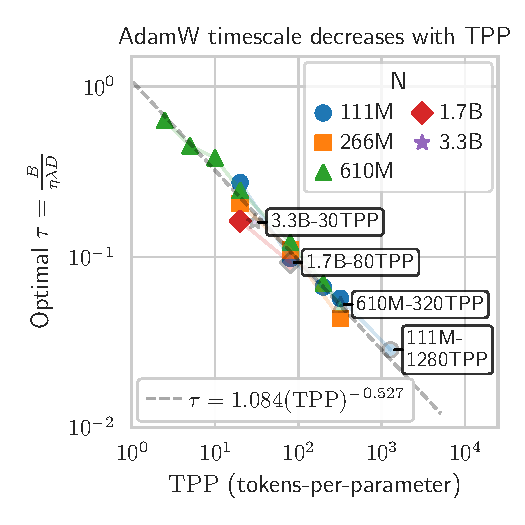
\includegraphics[trim={0.3cm 0.4cm 0.264cm 0.3cm}, clip, width=\linewidth]{pdffigs/tepoch_scaling_law.mydata.D2Z.pdf}
    \end{minipage}\hfill
    \begin{minipage}{0.33\textwidth}
        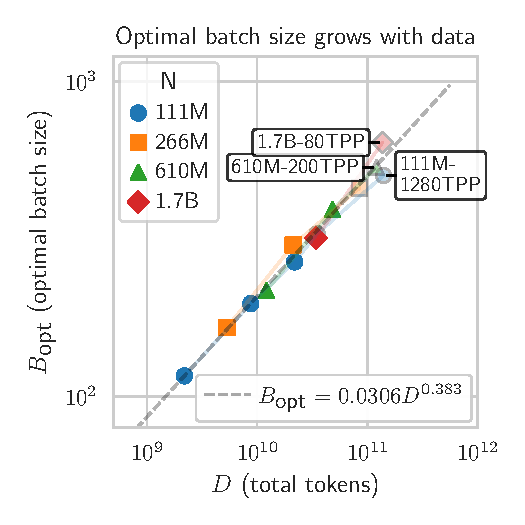
\includegraphics[trim={0.3cm 0.4cm 0.264cm 0.3cm}, clip, width=\linewidth]{pdffigs/bopt_scaling_law.mydata.D.pdf}
    \end{minipage}\hfill
    \begin{minipage}{0.33\textwidth}
        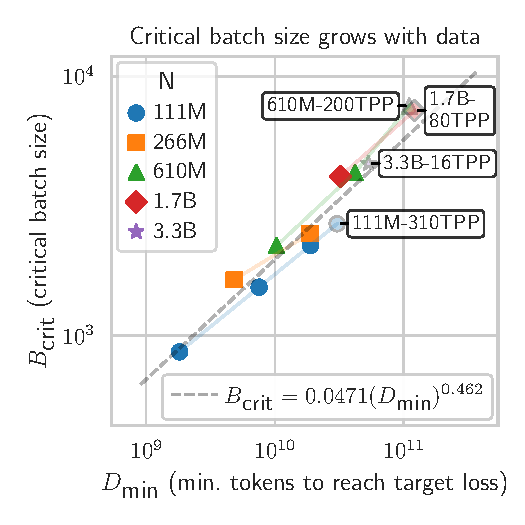
\includegraphics[trim={0.3cm 0.4cm 0.264cm 0.3cm}, clip, width=\linewidth]{pdffigs/loss_data.241005.cbs_scaling.Emin.pdf}
    \end{minipage}
    \caption{\textbf{Hyperparameters and their power lines}: Optimal
      $\tepoch$ obeys a power law in tokens-per-parameter
      ($\leftfig$), while optimal batch size ($\middlefig$) and
      critical batch size ($\rightfig$) obey power laws in
      $D$. \textcolor[rgb]{0.5,0.5,0.5}{Faded} markers indicate points
      not used in fitting; all fits generalize well to larger-scale
      runs.
      \label{fig:hook}}
\end{figure}
